\documentclass[11pt,a4paper,final]{article} %draft

\usepackage[T1,T2A]{fontenc}
\usepackage[utf8]{inputenc}
\usepackage[english, russian]{babel}

\usepackage[final]{pdfpages}

\usepackage{textcomp,enumitem}

\usepackage{amsmath,amsthm,amssymb}

\usepackage{fancyhdr} % для настройки страницы и колонтитулов

\usepackage{graphicx}

\usepackage{indentfirst} % автоматический отступ в начале каждого раздела

\usepackage[unicode, pdftex, colorlinks, urlcolor=blue]{hyperref}

\usepackage[left=2cm,right=2cm,top=2cm,bottom=2cm,bindingo ffset=0cm]{geometry}

\linespread{1.3} % устанавливает междустрочный интервал

\pagestyle{plain} % для отображения номеров внизу 

\usepackage{float}

\usepackage{listings} 

\usepackage{pdflscape}
\usepackage{listings} 
\definecolor{darkgreen}{rgb}{0,0.5,0}

\lstdefinelanguage{Haskell}{
	morekeywords={module, import, where, data, type, let, in, if, then, else, case, of, class, instance, deriving, do},
	sensitive=true,
	morecomment=[l]--,
	morecomment=[s]{\{-}{-\}},
	morestring=[b]",
}


\lstset{
	backgroundcolor=\color{white},  % Устанавливаем белый фон для блока кода
	basicstyle=\ttfamily\small\fontfamily{inconsolata}\selectfont,  % Основной стиль текста: моноширинный шрифт Inconsolata с небольшим размером
	commentstyle=\color{darkgreen}\slshape,  % Комментарии будут зелеными и курсивными
	keywordstyle=\color{blue}\bfseries,  % Ключевые слова выделяются синим цветом и полужирным шрифтом
	numberstyle=\scriptsize\color{gray},  % Стиль нумерации строк: маленький размер шрифта и серый цвет
	stringstyle=\color{orange},  % Строки (текст в кавычках) отображаются оранжевым цветом
	breakatwhitespace=false,  % Не прерывать строки только по пробелам
	breaklines=true,  % Автоматический перенос длинных строк
	postbreak=\mbox{\textcolor{gray}{$\hookrightarrow$}}, % Символ переноса строки
	captionpos=b,  % Позиция заголовка/описания для блока кода — внизу (b — bottom)
	keepspaces=true,  % Сохранить пробелы, как они есть, в исходном коде
	numbers=left,  % Нумерация строк будет отображаться слева
	numbersep=5pt,  % Отступ между строками кода и номерами строк (4pt)
	showspaces=false,  % Не показывать пробелы
	showstringspaces=false,  % Не показывать пробелы внутри строк
	showtabs=false,  % Не показывать символы табуляции
	tabsize=4,  % Размер табуляции — 4 пробела
	language=Haskell,  % Указываем язык программирования для синтаксического подсветки (C++)
	captionpos=t,  % Заголовок кода будет размещен вверху (t — top)
	xleftmargin=0mm,  % Убираем отступ слева
	frame=single,  % Однотонная рамка вокруг блока кода
	framerule=0.25mm,  % Толщина рамки — 0.25 мм
	literate=
	{а}{{\selectfont\char224}}1
	{б}{{\selectfont\char225}}1
	{в}{{\selectfont\char226}}1
	{г}{{\selectfont\char227}}1
	{д}{{\selectfont\char228}}1
	{е}{{\selectfont\char229}}1
	{ж}{{\selectfont\char230}}1
	{з}{{\selectfont\char231}}1
	{и}{{\selectfont\char232}}1
	{й}{{\selectfont\char233}}1
	{к}{{\selectfont\char234}}1
	{л}{{\selectfont\char235}}1
	{м}{{\selectfont\char236}}1
	{н}{{\selectfont\char237}}1
	{о}{{\selectfont\char238}}1
	{п}{{\selectfont\char239}}1
	{р}{{\selectfont\char240}}1
	{с}{{\selectfont\char241}}1
	{т}{{\selectfont\char242}}1
	{у}{{\selectfont\char243}}1
	{ф}{{\selectfont\char244}}1
	{х}{{\selectfont\char245}}1
	{ц}{{\selectfont\char246}}1
	{ч}{{\selectfont\char247}}1
	{ш}{{\selectfont\char248}}1
	{щ}{{\selectfont\char249}}1
	{ъ}{{\selectfont\char250}}1
	{ы}{{\selectfont\char251}}1
	{ь}{{\selectfont\char252}}1
	{э}{{\selectfont\char253}}1
	{ю}{{\selectfont\char254}}1
	{я}{{\selectfont\char255}}1
	{А}{{\selectfont\char192}}1
	{Б}{{\selectfont\char193}}1
	{В}{{\selectfont\char194}}1
	{Г}{{\selectfont\char195}}1
	{Д}{{\selectfont\char196}}1
	{Е}{{\selectfont\char197}}1
	{Ж}{{\selectfont\char198}}1
	{З}{{\selectfont\char199}}1
	{И}{{\selectfont\char200}}1
	{Й}{{\selectfont\char201}}1
	{К}{{\selectfont\char202}}1
	{Л}{{\selectfont\char203}}1
	{М}{{\selectfont\char204}}1
	{Н}{{\selectfont\char205}}1
	{О}{{\selectfont\char206}}1
	{П}{{\selectfont\char207}}1
	{Р}{{\selectfont\char208}}1
	{С}{{\selectfont\char209}}1
	{Т}{{\selectfont\char210}}1
	{У}{{\selectfont\char211}}1
	{Ф}{{\selectfont\char212}}1
	{Х}{{\selectfont\char213}}1
	{Ц}{{\selectfont\char214}}1
	{Ч}{{\selectfont\char215}}1
	{Ш}{{\selectfont\char216}}1
	{Щ}{{\selectfont\char217}}1
	{Ъ}{{\selectfont\char218}}1
	{Ы}{{\selectfont\char219}}1
	{Ь}{{\selectfont\char220}}1
	{Э}{{\selectfont\char221}}1
	{Ю}{{\selectfont\char222}}1
	{Я}{{\selectfont\char223}}1,
	numbers=left, % пронумеровать строки с левой стороны
	breaklines=true % разрешает автоматический перенос строк
}

\hypersetup{
	colorlinks=true, % делает ссылки цветными вместо рамки
	linkcolor=blue, % цвет внутренних ссылок
	urlcolor=blue, % цвет внешних ссылок
	citecolor=blue % цвет ссылок на литературу в тексте
}

\textheight=24cm 
\textwidth=16cm
\oddsidemargin=0pt 
\topmargin=-1.5cm
\parindent=24pt 
\parskip=0pt 
\tolerance=2000 
\flushbottom 

%\usepackage[font=scriptsize]{caption}
\usepackage[labelsep=period]{caption}

\usepackage{amsmath}
\usepackage{multirow} 
\usepackage{tabularx}

\newcommand{\specialcell}[2][l]{\begin{tabular}[#1]{@{}l@{}}#2\end{tabular}}

\begin{document}
	
\thispagestyle{empty}

\begin{center}
	{\Large МИНОБРНАУКИ РОССИИ}\\
	~\\
	{\large ФЕДЕРАЛЬНОЕ ГОСУДАРСТВЕННОЕ БЮДЖЕТНОЕ ОБРАЗОВАТЕЛЬНОЕ УЧРЕЖДЕНИЕ ВЫСШЕГО ПРОФЕССИОНАЛЬНОГО ОБРАЗОВАНИЯ}\\
	~\\
	{\Large \bf <<САНКТ-ПЕТЕРБУРГСКИЙ ПОЛИТЕХНИЧЕСКИЙ УНИВЕРСИТЕТ ПЕТРА ВЕЛИКОГО>>}\\
	~\\
	{\large Институт компьютерных наук и кибербезопасности }\\
	{\large Высшая школа технологий искусственного интеллекта}\\
	{\large Направление 02.03.01 Математика и компьютерные науки}\\
	~\\
	~\\
	~\\
	~\\
	{\Large \bf  Отчет по лабораторной работе №2 }\\
	\vspace{3mm}
	{\Large {по дисциплине <<Функциональное программирование>>}}\\
	\vspace{3mm}
	{\Large {Вариант 19}}\\
	~\\
	~\\
	~\\
	~\\
	~\\
	~\\
	{\large Обучающийся: \underline{\hspace{3.5cm}} \hspace{12mm} Шихалев А.О.}\\
	~\\
	{\large Руководитель: \underline{\hspace{3.5cm}} \hspace{12mm} Моторин Д.Е.}\\
	~\\
	~\\
	~\\
	~\\
	~\\
\end{center}
\begin{flushright}
	
	«\underline{\hspace{1cm}}»\underline{\hspace{3cm}}20\underline{\hspace{0.7cm}}г.
\end{flushright}
~\\
~\\
\begin{center}
	{\large Санкт-Петербург, 2024}
\end{center}

\newpage

\tableofcontents

\newpage
\section*{Введение}
\addcontentsline{toc}{section}{Введение}
Практическое задание №2 представляет собой реализацию двух программ:

\begin{enumerate}
	\item Вычислить все пары координат \((x, y)\) для заданного фрактала на глубину \(n\) шагов и вывести в виде списка списков пар (каждый уровень рекурсии является списком пар).
	
	\begin{center}
	\textbf{Фрактал: Папоротник Барнсли}
	\end{center}
	
	\item Реализовать заданную игру и стратегию следующим образом: в коде задать список, содержащий ходы пользователя; реализовать функцию, определяющую работу стратегии, и функцию, организующую игру (игра должна продолжаться не более 100 ходов).
	
	\begin{center}
		\textbf{Игра: Ним (N кучек в каждой не более M камней, игрок может взять неограниченное число камней)}
	\end{center}
	
\end{enumerate}

\par Лабораторная работа выполнена на языке Haskell в текстовом редакторе Visual Studio Code 1.95.3.


\newpage
\section{Математическое описание}
 \subsection{Фракталы}
Фрактал — множество, обладающее свойством самоподобия (объект, в точности или приближённо совпадающий с частью себя самого, то есть целое имеет ту же форму, что и одна или более частей). В математике под фракталами понимают множества точек в евклидовом пространстве, имеющие дробную метрическую размерность, либо метрическую размерность, отличную от топологической, поэтому их следует отличать от прочих геометрических фигур, ограниченных конечным числом звеньев. Самоподобные фигуры, повторяющиеся конечное число раз, называются предфракталами.


\subsection{Папоротник Барнсли}
Папоротник Барнсли — фрактал, названый в честь британского математика Майкла Барнсли, впервые описан в его книге <<Fractals Everywhere>>~\cite{barnsley}. Для его построения используется четыре простых трансформации, которые применяются случайным образом с определёнными вероятностями. Каждое преобразование масштабирует, поворачивает и смещает точки, начиная с одного начального положения. На каждом шаге, в зависимости от случайно выбранной трансформации, новая точка генерируется на основе предыдущей, и этот процесс повторяется многократно. Результатом становится изображение, напоминающее настоящие папоротники.

\[
\begin{aligned}
	T_1(x, y) &= \left( 0, 0.16y \right), \\
	T_2(x, y) &= \left( 0.85x + 0.04y, -0.04x + 0.85y + 1.6 \right), \\
	T_3(x, y) &= \left( 0.2x - 0.26y, 0.23x + 0.22y + 1.6 \right), \\
	T_4(x, y) &= \left( -0.15x + 0.28y, 0.26x + 0.24y + 0.44 \right).
\end{aligned}
\]

Каждое из этих преобразований применяется с вероятностью:
\[
P(T_1) = 0.01, \quad P(T_2) = 0.85, \quad P(T_3) = 0.07, \quad P(T_4) = 0.07.
\]

На рисунках 1-3 приведены примеры папоротника Барнсли для разного количества точек (n). Во всех примерах в качестве начальной была выбрана точка с координатами (0, 0).

\begin{figure}[H]
	\centering
	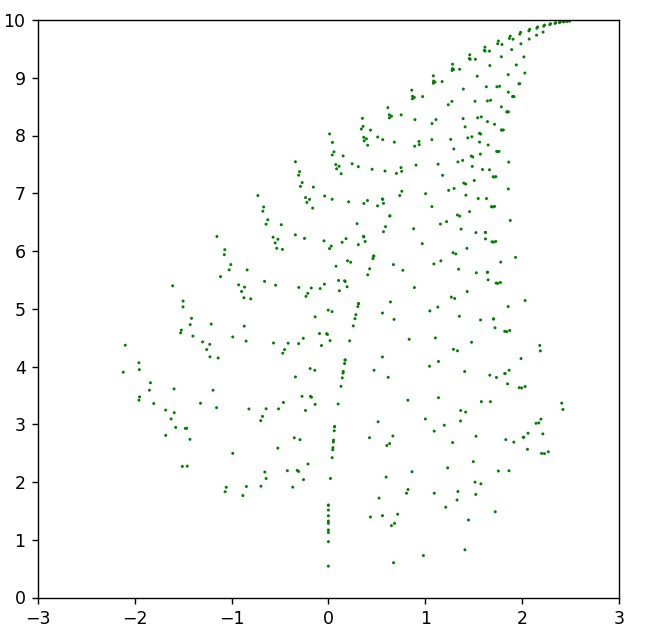
\includegraphics[width=0.6 \linewidth]{img/fern1.png}
	\caption{Папоротник Барнсли для n = 500.}
	\label{fig:fern500}
\end{figure}

\begin{figure}[H]
	\centering
	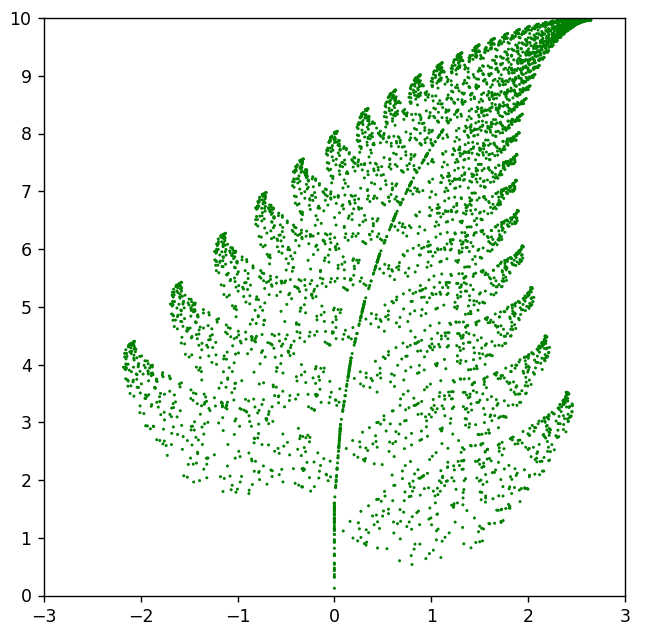
\includegraphics[width=0.6\linewidth]{img/fern2.png}
	\caption{Папоротник Барнсли для n = 5000.}
	\label{fig:fern5000}
\end{figure}

\begin{figure}[H]
	\centering
	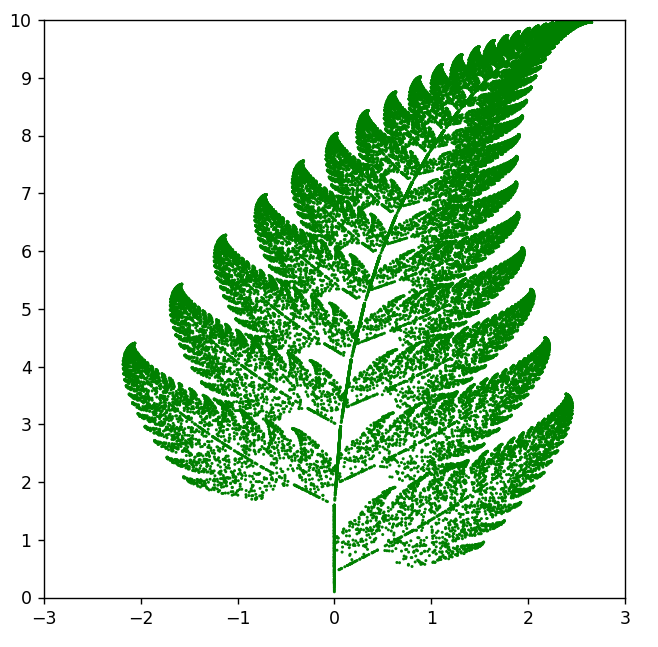
\includegraphics[width=0.6\linewidth]{img/fern3.png}
	\caption{Папоротник Барнсли для n = 50000.}
	\label{fig:fern50000}
\end{figure}


\subsection{Игра Ним}

\par Ним - игра, в которой два игрока по очереди берут предметы, разложеннные на есколько кучек. За один ход может быть взято любое количество предметов (больше нуля) из одной кучки. Выигрывает игрок, взявший последний предмет. В классическом варианте игры число кучек равняется трем. В нашем варианте кучек может быть произвольное число, не больше числа N.
В общем случае рассматривается p кучек камней с $N_1, N_2,...N_p$ камнями. Игроки ходят по очереди. Ход заключается в том, что игрок берёт из кучки i $\in$ [1,p], n $\in [1,N_i]$ предметов. Каждой позиции игры ставится в соответствие \textbf{ним-сумма} этой позиции — результат сложения размеров всех кучек в двоичной системе счисления без учёта переноса разрядов, то есть сложение двоичных разрядов чисел в поле вычетов по модулю 2: S = $N_1 \oplus N_2 \oplus ... \oplus N_p$

Выигрышная стратегия состоит в том, чтобы оставлять после своего хода позицию с ним-суммой, равной нулю. Она основана на том, что из любой позиции с ним-суммой, не равной нулю, можно одним ходом получить позицию с нулевой ним-суммой, а из позиции с нулевой ним-суммой любой ход ведёт в позицию с ним-суммой, отличной от нуля.

\newpage
\section{Особенности реализации}

\subsection{Папоротник Барнсли}

\subsubsection{Аффинные преобразование точек}

Функции, код которых представлен в листинге~\ref{lst:trfs}, реализуют четыре аффинных преобразования, используемых для построения фрактала папоротника Барнсли. Каждое преобразование принимает на вход точку в двумерном пространстве (координаты \( x \) и \( y \)) и возвращает новую точку, которая является результатом применения соответствующего преобразования.

\begin{lstlisting}[mathescape=true, caption={Аффинные преобразование точек}, label={lst:trfs}]
type Point = (Double, Double)
	
transformation1 :: Point -> Point
transformation1 (_, y) = (0, 0.16 * y)

transformation2 :: Point -> Point
transformation2 (x, y) = (0.85 * x + 0.04 * y, -0.04 * x + 0.85 * y + 1.6)

transformation3 :: Point -> Point
transformation3 (x, y) = (0.2 * x - 0.26 * y, 0.23 * x + 0.22 * y + 1.6)

transformation4 :: Point -> Point
transformation4 (x, y) = (-0.15 * x + 0.28 * y, 0.26 * x + 0.24 * y + 0.44)
\end{lstlisting}

\subsubsection{Генерация новой точки}

Генерация новой точки происходит с помощью функции \texttt{generateNextPoint} и вспомогательной функции \texttt{chooseTransformation}, код которых представлен в \hyperref[lst:genDot]{листинге 2}. \texttt{chooseTransformation} принимает на вход исходную точку и случайное число от 0 до 1, затем выбирает и применяет к точке трансформацию в соответствии с заданными вероятностями, и возвращает новую точку. \texttt{generateNextPoint} принимает на вход исходную точку и состояние генератора случайных чисел -- \texttt{g}, генерирует случайное число от 0 до 1, применяет функцию \texttt{applyTransformation} и возвращает пару -- новую точку и новое состояние генератора случайных чисел. 

\newpage
\begin{lstlisting}[caption={Код функций для генераций новых точек в папоротнике Барнсли.}, label={lst:genDot}]
import System.Random (randomR, mkStdGen, RandomGen, StdGen)
	
chooseTransformation :: Point -> Double -> Point
chooseTransformation point randValue
| randValue < 0.01 = transformation1 point
| randValue < 0.86 = transformation2 point
| randValue < 0.93 = transformation3 point
| otherwise = transformation4 point

generateNextPoint :: RandomGen g => Point -> g -> (Point, g)
generateNextPoint point gen = 
let (randValue, newGen) = randomR (0.0, 1.0) gen  -- генерируем случайное число
in (chooseTransformation point randValue, newGen)
\end{lstlisting}

\subsubsection{Рекурсивная генерация папоротника Барнсли}

Функция \texttt{barnsleyFern}, код которой представлен в \hyperref[lst:barnsleyFern]{листинге 3}, реализует рекурсивный алгоритм генерации списка точек, из которых состоит папоротник Барнсли. Функция принимает на вход текущее состояние генератора случайных чисел, начальную точку и число -- количество шагов рекурсии, а возвращает список точек папоротника Барнсли.

\begin{lstlisting}[caption={Код функции для построения папоротника Барнсли.}, label={lst:barnsleyFern}]
buildFern :: RandomGen g => Point -> Int -> g -> [Point]
buildFern _ 0 _ = []
buildFern currentPoint steps gen =
let (nextPoint, newGen) = generateNextPoint currentPoint gen
remainingPoints = buildFern nextPoint (steps - 1) newGen
in currentPoint : remainingPoints        
\end{lstlisting}


\subsection{Реализация игры «Ним»}

\subsubsection{Инициализация игры}

Функция \texttt{initializeGame}, представлена в листинге \hyperref[lst:init]{листинге 4}, позволяет задать начальное состояние игры. Пользователь вводит количество куч и количество камней в каждой из них. Если ввод данных не совпадает с указанным количеством куч, функция вызывает себя рекурсивно, чтобы исправить ошибку ввода.

\begin{lstlisting}[caption={Инициализация игры}, label={lst:init}]
initializeGame :: IO GameState
initializeGame = do
putStrLn "Введите количество куч:"
nPiles <- read <$> getLine
putStrLn "Введите количество камней в каждой куче (через пробел):"
stones <- map read . words <$> getLine
if length stones == nPiles
then return stones
else do
putStrLn "Ошибка: количество куч не совпадает с введенными значениями."
initializeGame
\end{lstlisting}

\subsubsection{Проверка окончания игры}

Функция \texttt{isGameOver}, приведенная в листинге \hyperref[lst:isGameOver]{листинге 5}, проверяет, завершена ли игра, возвращая \texttt{True}, если все кучи пусты.

\begin{lstlisting}[caption={Проверка окончания игры}, label={lst:isGameOver}]
isGameOver :: GameState -> Bool
isGameOver = all (== 0)
\end{lstlisting}

\subsection{Ходы игроков}

Функция \texttt{playerMove}, представлена в листинге \hyperref[lst:playerMove]{листинге 6}, позволяет пользователю сделать ход. Игрок выбирает кучу и количество камней, которые хочет взять. Если введенные данные некорректны, функция повторяет запрос ввода.

\begin{lstlisting}[caption={Ход игрока}, label={lst:playerMove}]
playerMove :: GameState -> IO (Int, Int)
playerMove piles = do
printGameState piles
putStrLn "Выберите номер кучи (начиная с 1):"
pile <- read <$> getLine
putStrLn "Сколько камней вы хотите взять?"
stones <- read <$> getLine
if pile > 0 && pile <= length piles && stones > 0 && stones <= piles !! (pile - 1)
then return (pile - 1, stones)
else do
putStrLn "Неверный ход. Попробуйте снова."
playerMove piles
\end{lstlisting}

Функция \texttt{computerMove}, представлена в \hyperref[lst:computerMove]{листинге 7}, реализует стратегию компьютера на основе Nim-суммы. Если Nim-сумма равна нулю, компьютер выбирает любой допустимый ход. В противном случае он совершает выигрышный ход, уменьшая количество камней в одной из куч.

\begin{lstlisting}[caption={Ход компьютера}, label={lst:computerMove}]
computerMove :: GameState -> IO (Int, Int)
computerMove piles = do
let nimSum = foldr xor 0 piles
let moves = [(i, 1) | (i, s) <- zip [0..] piles, s > 0]
let winningMoves = [(i, s - (s `xor` nimSum)) | (i, s) <- zip [0..] piles, s `xor` nimSum < s]

let move = if nimSum == 0 
then case moves of 
(x:_) -> x 
[]    -> error "Нет возможных ходов" 
else case winningMoves of 
(x:_) -> x
[]    -> error "Нет выигрышных ходов" 

let (pile, stones) = move
putStrLn $ "Компьютер выбрал кучу " ++ show (pile + 1) ++ " и взял " ++ show stones ++ " камней."
return move
\end{lstlisting}

\subsubsection{Обновление состояния игры}

Функция \texttt{makeMove}, приведенная в листинге \hyperref[lst:makeMove]{листинге 8}, обновляет состояние игры после хода, уменьшая количество камней в выбранной куче.

\begin{lstlisting}[caption={Обновление состояния игры}, label={lst:makeMove}]
makeMove :: GameState -> (Int, Int) -> GameState
makeMove piles (pile, stones) = 
take pile piles ++ [piles !! pile - stones] ++ drop (pile + 1) piles
\end{lstlisting}

\subsection{Основная логика игры}

Функция \texttt{playNim}, приведенная в листинге~\ref{lst:playNim}, организует игровой процесс. Она последовательно обрабатывает ходы игрока и компьютера, обновляет состояние игры и завершает игру, когда все кучи пусты.

\begin{lstlisting}[caption={Основная логика игры}, label={lst:playNim}]
playNim :: GameState -> MoveHistory -> IO ()
playNim piles moves
| isGameOver piles = do
putStrLn "Игра окончена!"
printMoveHistory moves
| otherwise = do
(pile, stones) <- playerMove piles
let newPiles = makeMove piles (pile, stones)
let newMoves = moves ++ [("Вы", pile, stones)]
if isGameOver newPiles
then do
putStrLn "Поздравляем, вы выиграли!"
printMoveHistory newMoves
else do
(pileComp, stonesComp) <- computerMove newPiles
let finalPiles = makeMove newPiles (pileComp, stonesComp)
let finalMoves = newMoves ++ [("Компьютер", pileComp, stonesComp)]
if isGameOver finalPiles
then do
putStrLn "Компьютер выиграл!"
printMoveHistory finalMoves
else playNim finalPiles finalMoves
\end{lstlisting}

\newpage
\section{Результаты работы программы}

На \hyperref[fig:pic1]{рисунке 4} демонстрируется работа программы для генерации точек папоротника Барнсли на примере с 20 точками.

На \hyperref[fig:pic2]{рисунке 5} представлена работа программы игры Ним. 


\begin{figure}[H]
	\centering
	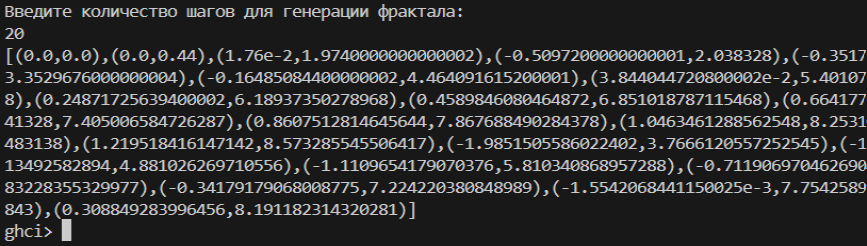
\includegraphics[width=0.8 \linewidth]{img/pic1.png}
	\caption{Результат запуска программы для генерации точек папоротника Барнсли}
	\label{fig:pic1}
\end{figure}

\begin{figure}[H]
	\centering
	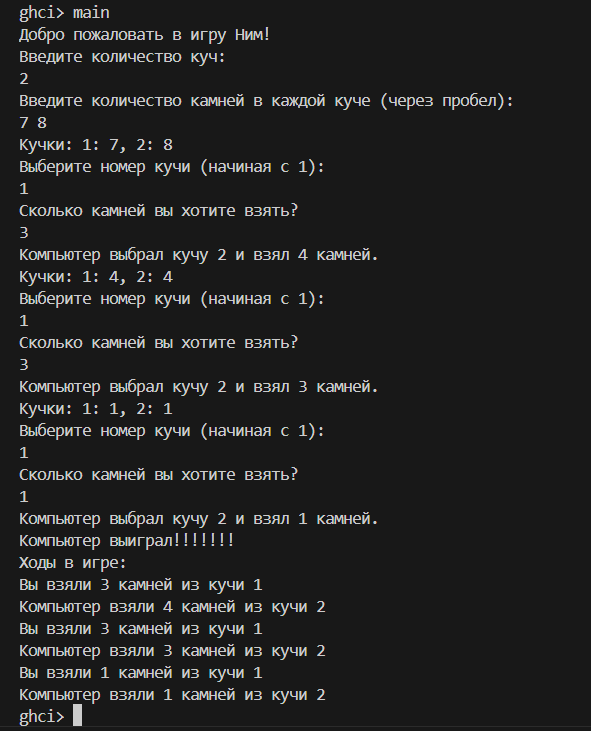
\includegraphics[width=0.6 \linewidth]{img/pic2.png}
	\caption{Результат работы программы игры Ним}
	\label{fig:pic2}
\end{figure}


\section*{Заключение}
\addcontentsline{toc}{section}{Заключение}

В ходе выполнения лабораторной работы были реализованы две программы на языке программирования Haskell. Первая программа генерирует точки для папоротника Барнсли с помощью рекурсивного алгоритма с заданным количеством шагов рекурсии. Вторая программа реализует классическую игру <<Ним>>, в которой игрок и компьютер поочередно делают ходы. Для каждой задачи был сформирован (.hs) файл, содержащий реализацию.


\newpage
\section*{Список литературы}
\addcontentsline{toc}{section}{Список литературы} % Добавляем раздел в содержание

\begin{enumerate}[label={[\arabic*]}]
	\item Курт У. Программируй на Haskell / пер. с англ. С. Соловьева. — Москва: ДМК Пресс, 2019. — 384 с.
	
	\item Barnsley M.F. Fractals Everywhere. — Academic Press, 1988. — 394 p. ISBN-13 \href{https://isbnsearch.org/isbn/9780120790616}{978-0-12-079061-6}
	
	\item Bouton C.L. Nim, a game with a complete mathematical theory // Annals of Mathematics. — 1901. — Vol. 3, No. 1. — P. 35–39. DOI \href{https://doi.org/10.2307/1967631}{10.2307/1967631}.
\end{enumerate}



\end{document}